% generated by Plantuml 1.2024.4       
\definecolor{plantucolor0000}{RGB}{241,241,241}
\definecolor{plantucolor0001}{RGB}{24,24,24}
\definecolor{plantucolor0002}{RGB}{173,209,178}
\definecolor{plantucolor0003}{RGB}{0,0,0}
\definecolor{plantucolor0004}{RGB}{200,41,48}
\definecolor{plantucolor0005}{RGB}{3,128,72}
\definecolor{plantucolor0006}{RGB}{132,190,132}
\scalebox{0.8466}{
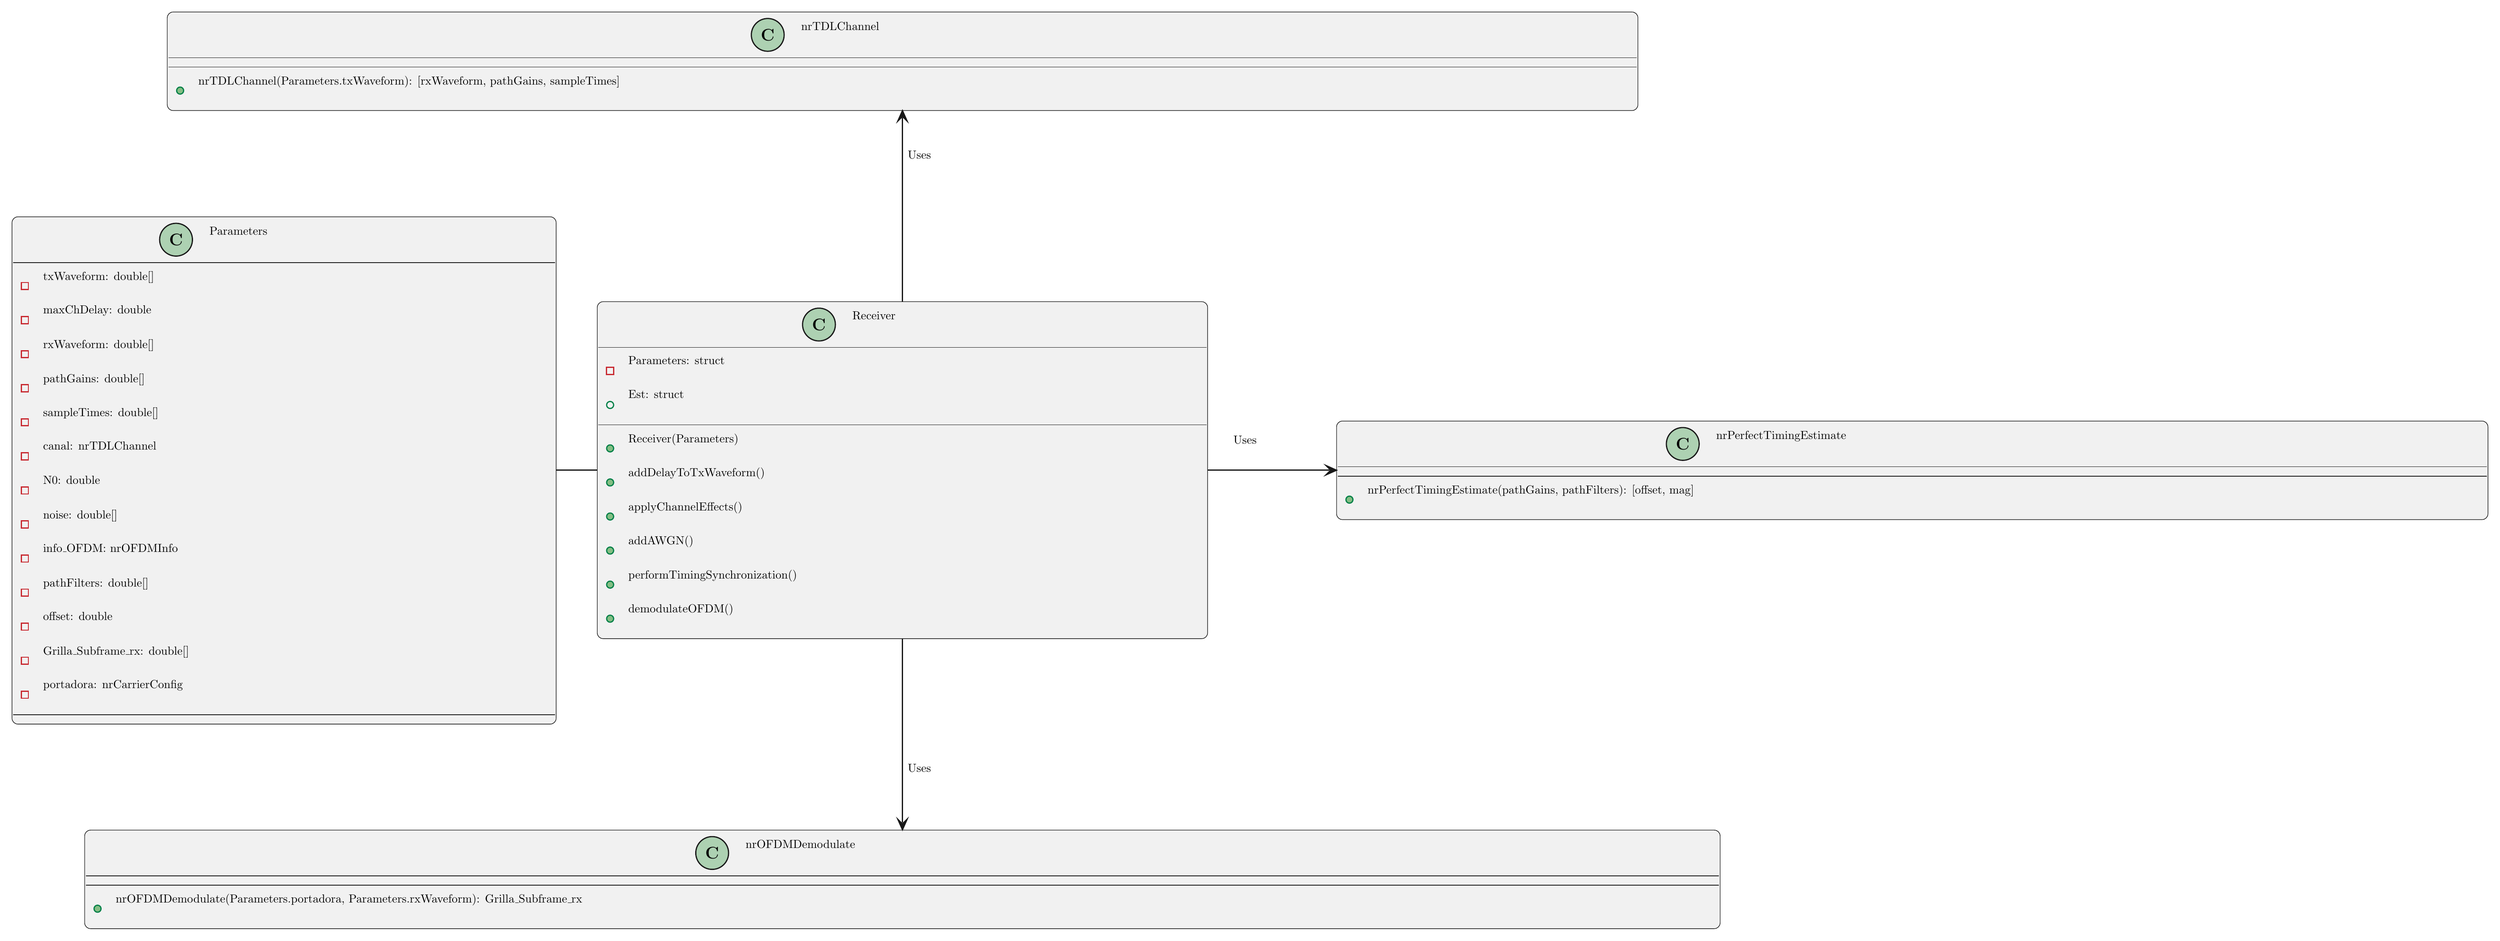
\begin{tikzpicture}[yscale=-1
,pstyle0/.style={color=plantucolor0001,fill=plantucolor0000,line width=0.5pt}
,pstyle1/.style={color=plantucolor0001,fill=plantucolor0002,line width=1.0pt}
,pstyle2/.style={color=plantucolor0001,line width=0.5pt}
,pstyle3/.style={color=plantucolor0004,line width=1.0pt}
,pstyle5/.style={color=plantucolor0005,fill=plantucolor0006,line width=1.0pt}
,pstyle6/.style={color=plantucolor0001,line width=1.0pt}
,pstyle7/.style={color=plantucolor0001,fill=plantucolor0001,line width=1.0pt}
]
\draw[pstyle0] (506.5pt,259.5pt) arc (180:270:5pt) -- (511.5pt,254.5pt) -- (1022.4588pt,254.5pt) arc (270:360:5pt) -- (1027.4588pt,259.5pt) -- (1027.4588pt,537.4141pt) arc (0:90:5pt) -- (1022.4588pt,542.4141pt) -- (511.5pt,542.4141pt) arc (90:180:5pt) -- (506.5pt,537.4141pt) -- cycle;
\draw[pstyle1] (695.7437pt,274.0508pt) ellipse (14pt and 14pt);
\node at (695.7437pt,274.0508pt)[]{\textbf{\Large C}};
\node at (720.7437pt,259.5pt)[below right,color=black]{Receiver};
\draw[pstyle2] (507.5pt,293.6016pt) -- (1026.4588pt,293.6016pt);
\draw[pstyle3] (514.5pt,310.6523pt) rectangle (520.5pt,316.6523pt);
\node at (529.5pt,297.6016pt)[below right,color=black]{Parameters: struct};
\draw[color=plantucolor0005,line width=1.0pt] (517.5pt,342.7539pt) ellipse (3pt and 3pt);
\node at (529.5pt,326.7031pt)[below right,color=black]{Est: struct};
\draw[pstyle2] (507.5pt,359.8047pt) -- (1026.4588pt,359.8047pt);
\draw[pstyle5] (517.5pt,379.8555pt) ellipse (3pt and 3pt);
\node at (529.5pt,363.8047pt)[below right,color=black]{Receiver(Parameters)};
\draw[pstyle5] (517.5pt,408.957pt) ellipse (3pt and 3pt);
\node at (529.5pt,392.9063pt)[below right,color=black]{addDelayToTxWaveform()};
\draw[pstyle5] (517.5pt,438.0586pt) ellipse (3pt and 3pt);
\node at (529.5pt,422.0078pt)[below right,color=black]{applyChannelEffects()};
\draw[pstyle5] (517.5pt,467.1602pt) ellipse (3pt and 3pt);
\node at (529.5pt,451.1094pt)[below right,color=black]{addAWGN()};
\draw[pstyle5] (517.5pt,496.2617pt) ellipse (3pt and 3pt);
\node at (529.5pt,480.2109pt)[below right,color=black]{performTimingSynchronization()};
\draw[pstyle5] (517.5pt,525.3633pt) ellipse (3pt and 3pt);
\node at (529.5pt,509.3125pt)[below right,color=black]{demodulateOFDM()};
\draw[pstyle0] (7pt,187pt) arc (180:270:5pt) -- (12pt,182pt) -- (466.4287pt,182pt) arc (270:360:5pt) -- (471.4287pt,187pt) -- (471.4287pt,610.4219pt) arc (0:90:5pt) -- (466.4287pt,615.4219pt) -- (12pt,615.4219pt) arc (90:180:5pt) -- (7pt,610.4219pt) -- cycle;
\draw[pstyle1] (146.9954pt,201.5508pt) ellipse (14pt and 14pt);
\node at (146.9954pt,201.5508pt)[]{\textbf{\Large C}};
\node at (171.9954pt,187pt)[below right,color=black]{Parameters};
\draw[pstyle2] (8pt,221.1016pt) -- (470.4287pt,221.1016pt);
\draw[pstyle3] (15pt,238.1523pt) rectangle (21pt,244.1523pt);
\node at (30pt,225.1016pt)[below right,color=black]{txWaveform: double[]};
\draw[pstyle3] (15pt,267.2539pt) rectangle (21pt,273.2539pt);
\node at (30pt,254.2031pt)[below right,color=black]{maxChDelay: double};
\draw[pstyle3] (15pt,296.3555pt) rectangle (21pt,302.3555pt);
\node at (30pt,283.3047pt)[below right,color=black]{rxWaveform: double[]};
\draw[pstyle3] (15pt,325.457pt) rectangle (21pt,331.457pt);
\node at (30pt,312.4063pt)[below right,color=black]{pathGains: double[]};
\draw[pstyle3] (15pt,354.5586pt) rectangle (21pt,360.5586pt);
\node at (30pt,341.5078pt)[below right,color=black]{sampleTimes: double[]};
\draw[pstyle3] (15pt,383.6602pt) rectangle (21pt,389.6602pt);
\node at (30pt,370.6094pt)[below right,color=black]{canal: nrTDLChannel};
\draw[pstyle3] (15pt,412.7617pt) rectangle (21pt,418.7617pt);
\node at (30pt,399.7109pt)[below right,color=black]{N0: double};
\draw[pstyle3] (15pt,441.8633pt) rectangle (21pt,447.8633pt);
\node at (30pt,428.8125pt)[below right,color=black]{noise: double[]};
\draw[pstyle3] (15pt,470.9648pt) rectangle (21pt,476.9648pt);
\node at (30pt,457.9141pt)[below right,color=black]{info\_OFDM: nrOFDMInfo};
\draw[pstyle3] (15pt,500.0664pt) rectangle (21pt,506.0664pt);
\node at (30pt,487.0156pt)[below right,color=black]{pathFilters: double[]};
\draw[pstyle3] (15pt,529.168pt) rectangle (21pt,535.168pt);
\node at (30pt,516.1172pt)[below right,color=black]{offset: double};
\draw[pstyle3] (15pt,558.2695pt) rectangle (21pt,564.2695pt);
\node at (30pt,545.2188pt)[below right,color=black]{Grilla\_Subframe\_rx: double[]};
\draw[pstyle3] (15pt,587.3711pt) rectangle (21pt,593.3711pt);
\node at (30pt,574.3203pt)[below right,color=black]{portadora: nrCarrierConfig};
\draw[pstyle2] (8pt,607.4219pt) -- (470.4287pt,607.4219pt);
\draw[pstyle0] (139.5pt,12pt) arc (180:270:5pt) -- (144.5pt,7pt) -- (1389.7052pt,7pt) arc (270:360:5pt) -- (1394.7052pt,12pt) -- (1394.7052pt,86.2031pt) arc (0:90:5pt) -- (1389.7052pt,91.2031pt) -- (144.5pt,91.2031pt) arc (90:180:5pt) -- (139.5pt,86.2031pt) -- cycle;
\draw[pstyle1] (652.0203pt,26.5508pt) ellipse (14pt and 14pt);
\node at (652.0203pt,26.5508pt)[]{\textbf{\Large C}};
\node at (677.0203pt,12pt)[below right,color=black]{nrTDLChannel};
\draw[pstyle2] (140.5pt,46.1016pt) -- (1393.7052pt,46.1016pt);
\draw[pstyle2] (140.5pt,54.1016pt) -- (1393.7052pt,54.1016pt);
\draw[pstyle5] (150.5pt,74.1523pt) ellipse (3pt and 3pt);
\node at (162.5pt,58.1016pt)[below right,color=black]{nrTDLChannel(Parameters.txWaveform): [rxWaveform, pathGains, sampleTimes]};
\draw[pstyle0] (69pt,711pt) arc (180:270:5pt) -- (74pt,706pt) -- (1459.8892pt,706pt) arc (270:360:5pt) -- (1464.8892pt,711pt) -- (1464.8892pt,785.2031pt) arc (0:90:5pt) -- (1459.8892pt,790.2031pt) -- (74pt,790.2031pt) arc (90:180:5pt) -- (69pt,785.2031pt) -- cycle;
\draw[pstyle1] (604.5927pt,725.5508pt) ellipse (14pt and 14pt);
\node at (604.5927pt,725.5508pt)[]{\textbf{\Large C}};
\node at (629.5927pt,711pt)[below right,color=black]{nrOFDMDemodulate};
\draw[pstyle2] (70pt,745.1016pt) -- (1463.8892pt,745.1016pt);
\draw[pstyle2] (70pt,753.1016pt) -- (1463.8892pt,753.1016pt);
\draw[pstyle5] (80pt,773.1523pt) ellipse (3pt and 3pt);
\node at (92pt,757.1016pt)[below right,color=black]{nrOFDMDemodulate(Parameters.portadora, Parameters.rxWaveform): Grilla\_Subframe\_rx};
\draw[pstyle0] (1137.5pt,361.5pt) arc (180:270:5pt) -- (1142.5pt,356.5pt) -- (2115.2267pt,356.5pt) arc (270:360:5pt) -- (2120.2267pt,361.5pt) -- (2120.2267pt,435.7031pt) arc (0:90:5pt) -- (2115.2267pt,440.7031pt) -- (1142.5pt,440.7031pt) arc (90:180:5pt) -- (1137.5pt,435.7031pt) -- cycle;
\draw[pstyle1] (1432.9925pt,376.0508pt) ellipse (14pt and 14pt);
\node at (1432.9925pt,376.0508pt)[]{\textbf{\Large C}};
\node at (1457.9925pt,361.5pt)[below right,color=black]{nrPerfectTimingEstimate};
\draw[pstyle2] (1138.5pt,395.6016pt) -- (2119.2267pt,395.6016pt);
\draw[pstyle2] (1138.5pt,403.6016pt) -- (2119.2267pt,403.6016pt);
\draw[pstyle5] (1148.5pt,423.6523pt) ellipse (3pt and 3pt);
\node at (1160.5pt,407.6016pt)[below right,color=black]{nrPerfectTimingEstimate(pathGains, pathFilters): [offset, mag]};
\draw[pstyle6] (471.03pt,398.5pt) ..controls (482.79pt,398.5pt) and (494.54pt,398.5pt) .. (506.29pt,398.5pt);
\draw[pstyle6] (767pt,97.23pt) ..controls (767pt,137.59pt) and (767pt,195.44pt) .. (767pt,254.42pt);
\draw[pstyle7] (767pt,91.23pt) -- (763pt,100.23pt) -- (767pt,96.23pt) -- (771pt,100.23pt) -- (767pt,91.23pt) -- cycle;
\node at (768pt,122pt)[below right,color=black]{Uses};
\draw[pstyle6] (767pt,542.6pt) ..controls (767pt,601.53pt) and (767pt,659.31pt) .. (767pt,699.68pt);
\draw[pstyle7] (767pt,705.68pt) -- (771pt,696.68pt) -- (767pt,700.68pt) -- (763pt,696.68pt) -- (767pt,705.68pt) -- cycle;
\node at (768pt,646pt)[below right,color=black]{Uses};
\draw[pstyle6] (1027.67pt,398.5pt) ..controls (1062.86pt,398.5pt) and (1093.85pt,398.5pt) .. (1131.47pt,398.5pt);
\draw[pstyle7] (1137.47pt,398.5pt) -- (1128.47pt,394.5pt) -- (1132.47pt,398.5pt) -- (1128.47pt,402.5pt) -- (1137.47pt,398.5pt) -- cycle;
\node at (1046pt,365.5pt)[below right,color=black]{Uses};
\end{tikzpicture}
}
